\documentclass[aspectratio=169]{beamer}

\usepackage{ccicons}
\usepackage{fontspec}
\usepackage{listings}
\usepackage{tikz}
\usepackage{svg}

\definecolor{uclablue}{RGB}{39,116,174}
\definecolor{uclagold}{RGB}{255,179,0}

\definecolor{ubcorange}{RGB}{158, 66, 37}

\definecolor{cugold}{RGB}{207, 184, 124}
\definecolor{cudarkgray}{RGB}{86, 90, 92}

\definecolor{solarizedred}{RGB}{220, 50, 47}
\definecolor{solarizedblue}{RGB}{38, 139, 210}
\definecolor{solarizedgreen}{RGB}{133, 153, 0}
\definecolor{solarizedpurple}{RGB}{108, 113, 196}
\definecolor{solarizedmagenta}{RGB}{211, 54, 130}

\definecolor{pantone655}{RGB}{0, 42, 92}
\definecolor{pantone7453}{RGB}{123, 164, 217}
\definecolor{pantone633}{RGB}{0, 139, 176}
\definecolor{pantone7492}{RGB}{218, 229, 205}

\colorlet{primarycolor}{pantone655}
\colorlet{secondarycolor}{pantone7453}


\usetikzlibrary{
  arrows,
  arrows.meta,
  automata,
  backgrounds,
  calc,
  chains,
  decorations.pathreplacing,
  fit,
  intersections,
  matrix,
  overlay-beamer-styles,
  positioning,
  shapes,
  shapes.multipart,
  tikzmark,
}
\usetikzmarklibrary{listings}

\hypersetup{
  colorlinks=true,
  urlcolor=cudarkgray,
}

\setbeamercolor{frametitle}{fg=primarycolor}
\setbeamercolor{structure}{fg=primarycolor}
\setbeamercolor{enumerate item}{fg=black}
\setbeamercolor{itemize item}{fg=black}
\setbeamercolor{itemize subitem}{fg=black}

\setbeamersize{text margin left=26.6mm}
\addtolength{\headsep}{2mm}

\setbeamertemplate{navigation symbols}{}
\setbeamertemplate{headline}{}
\setbeamertemplate{footline}{}
\setbeamertemplate{itemize item}{\color{black}}
\setbeamertemplate{itemize items}[circle]

\setbeamertemplate{footline}{
  \begin{tikzpicture}[remember picture,
                      overlay,
                      shift={(current page.south west)}]
    \node [black!50, inner sep=2mm, anchor=south east]
          at (current page.south east) {\footnotesize \insertframenumber};
  \end{tikzpicture}
}

\setsansfont{Inter}[Scale=MatchLowercase]
\setmonofont{Hack}[Scale=MatchLowercase]

\makeatletter
\newcommand\version[1]{\renewcommand\@version{#1}}
\newcommand\@version{}
\def\insertversion{\@version}

\newcommand\lecturenumber[1]{\renewcommand\@lecturenumber{#1}}
\newcommand\@lecturenumber{}
\def\insertlecturenumber{\@lecturenumber}
\makeatother

\setbeamertemplate{title page}
{
  \begin{tikzpicture}[remember picture,
                      overlay,
                      shift={(current page.south west)},
                      background rectangle/.style={fill=pantone655},
                      show background rectangle]
    \node [anchor=west, align=left, inner sep=0, text=white]
          (lecturenumber) at (\paperwidth / 6, \paperheight * 3 / 4)
          {\Large Lecture \insertlecturenumber};
    \node [inner sep=0, align=left, text=white, node distance=0,
          above left=of lecturenumber, anchor=south west, yshift=2mm]
          {\Large ECE 344: Operating Systems};
    \node (title) [inner sep=0, anchor=west, align=left, text=white,
                   text width=30em]
          at (\paperwidth / 6, \paperheight / 2)
          {{\bfseries \Huge \inserttitle{}}};
    \node [inner sep=0, align=right, text=white, node distance=0,
          below right=of title, anchor=north east, yshift=-1mm]
          {{\footnotesize \ttfamily \insertversion}};
    \node [inner sep=0, text=white, align=left, anchor=west]
          (author) at (\paperwidth / 6, \paperheight / 4)
          {\insertauthor};
    \node [text=white, inner sep=0, align=left, node distance=0,
           below left=of author, anchor=north west, yshift=-2mm]
          {\insertdate};
    \node [align=right, anchor=south east, inner sep=2mm, text=white]
          (license) at (\paperwidth, 0)
          {\footnotesize This  work is licensed under a
           \href{http://creativecommons.org/licenses/by-sa/4.0/}
                {\color{pantone7453} Creative Commons Attribution-ShareAlike 4.0
                 International License}};
    \node [text=white, inner sep=0, align=right, node distance=0,
           above right=of license, anchor=south east, xshift=-2mm]
          {\Large \ccbysa};
  \end{tikzpicture}
}

\tikzset{
  >=Straight Barb[],
  shorten >=1pt,
  initial text=,
}

\lstset{
  basicstyle=\footnotesize\ttfamily,
  language=C,
  escapechar=@,
  commentstyle=\color{black!50},
}


\lecturenumber{22}
\title{Clock Page Replacement}
\version{1.0.0}
\author{Jon Eyolfson}
\date{November 1/2, 2021}

\tikzset{swapin/.style args = {(#1,#2)}{%
    row #1 column #2/.style={nodes={text=red}}}}

\begin{document}
  \begin{frame}[plain, noframenumbering]
    \titlepage
  \end{frame}

  \begin{frame}
    \frametitle{Clock Algorithm}

    Data structures:
    \begin{itemize}
      \item Keeps a circular list of pages in memory
      \item Uses a reference bit for each page in memory (light grey in next slides)
      \item Has a ``hand'' (iterator) pointing to the last element examined
    \end{itemize}

    \vspace{2em}

    Algorithm, to insert a new page:
    \begin{itemize}
      \item Check the hand's reference bit, if it's 0 then place the page and advance hand
      \item If the reference bit is 1, set it to 0, advance the hand, and repeat
    \end{itemize}

    \vspace{2em}

    For page accesses, set the reference bit to 1
  \end{frame}

  \begin{frame}[fragile]
    \frametitle{Clock Example (with Diagram)}

    Assume our physical memory can only hold 4 pages, and we access the following:

    \hspace{2em} 1 2 3 4 5 2 3 1 2 3 (all of the pages are initially on disk)

    \begin{center}
      \begin{tikzpicture}
        \matrix (m) [
          matrix of nodes,
          nodes in empty cells,
          minimum width=2em,
          minimum height=2em,
          align=center,
          column sep=1em,
          column 1/.style={visible on=<2->},
          column 2/.style={visible on=<3->},
          column 3/.style={visible on=<4->},
          column 4/.style={visible on=<5->},
          column 5/.style={visible on=<6->},
          column 6/.style={visible on=<11->},
          column 7/.style={visible on=<12->},
          column 8/.style={visible on=<13->},
          column 9/.style={visible on=<16->},
          column 10/.style={visible on=<17->},
        ] {
          1 & 2 & 3 & 4 & 5 & 2 & 3 & 1 & 2 & 3 \\
        };
      \end{tikzpicture}

      \vspace{1em}

      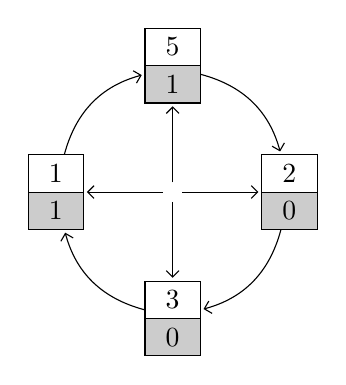
\begin{tikzpicture}[
        box/.style={
          draw,
          align=center,
          minimum width=2em,
          minimum height=6em,
          rectangle split,
          rectangle split parts=2,
          rectangle split part fill={white, black!20},
        }
      ]

        \node (c) at (0, 0) {};

        \node<1> [above=of c, box] (n) {0 \nodepart{second} 0};
        \node<2-5> [above=of c, box] {1 \nodepart{second} 1};
        \node<6-9> [above=of c, box] {1 \nodepart{second} 0};
        \node<10-> [above=of c, box] {5 \nodepart{second} 1};

        \node<1-2> [right=of c, box] (e) {0 \nodepart{second} 0};
        \node<3-6,11-12,16-> [right=of c, box] {2 \nodepart{second} 1};
        \node<7-10,13-15> [right=of c, box] {2 \nodepart{second} 0};

        \node<1-3> [below=of c, box] (s) {0 \nodepart{second} 0};
        \node<4-7,12-13,17-> [below=of c, box] {3 \nodepart{second} 1};
        \node<8-11,14-16> [below=of c, box] {3 \nodepart{second} 0};

        \node<1-4> [left=of c, box] (w) {0 \nodepart{second} 0};
        \node<5-8> [left=of c, box] (w) {4 \nodepart{second} 1};
        \node<9-14> [left=of c, box] (w) {4 \nodepart{second} 0};
        \node<15-> [left=of c, box] (w) {1 \nodepart{second} 1};

        \path [->] (n) edge [bend left] (e)
                   (e) edge [bend left] (s)
                   (s) edge [bend left] (w)
                   (w) edge [bend left] (n);

        \path<1,5,9,15-> [->] (c) edge (n);
        \path<2,6,10-12> [->] (c) edge (e);
        \path<3,7,13> [->] (c) edge (s);
        \path<4,8,14> [->] (c) edge (w);

      \end{tikzpicture}
    \end{center}
  \end{frame}

  \begin{frame}[fragile]
    \frametitle{Clock Example}

    Assume our physical memory can only hold 4 pages, and we access the following:

    \hspace{2em} 1 2 3 4 5 2 3 1 2 3 (all of the pages are initially on disk)

    \begin{center}
      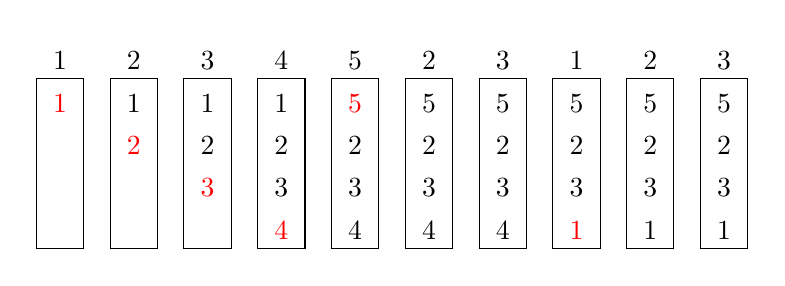
\begin{tikzpicture}[
        every node/.style={
          align=center,
          text height=2ex,
          text width=1em
        },
        swapin/.list={
          (2,1),
          (3,2),
          (4,3),
          (5,4),
          (2,5),
          (5,8)
        },
      ]
        \matrix (m) [
          matrix of nodes,
          nodes in empty cells,
          column sep=1em,
          column 2/.style={visible on=<2->},
          column 3/.style={visible on=<3->},
          column 4/.style={visible on=<4->},
          column 5/.style={visible on=<5->},
          column 6/.style={visible on=<6->},
          column 7/.style={visible on=<7->},
          column 8/.style={visible on=<8->},
          column 9/.style={visible on=<9->},
          column 10/.style={visible on=<10->},
        ] {
          1 & 2 & 3 & 4 & 5 & 2 & 3 & 1 & 2 & 3 \\
          1 & 1 & 1 & 1 & 5 & 5 & 5 & 5 & 5 & 5 \\
            & 2 & 2 & 2 & 2 & 2 & 2 & 2 & 2 & 2 \\
            &   & 3 & 3 & 3 & 3 & 3 & 3 & 3 & 3 \\
            &   &   & 4 & 4 & 4 & 4 & 1 & 1 & 1 \\
        };
        \draw (m-2-1.north west) rectangle (m-5-1.south east);
        \draw (m-2-2.north west) rectangle (m-5-2.south east);
        \draw (m-2-3.north west) rectangle (m-5-3.south east);
        \draw (m-2-4.north west) rectangle (m-5-4.south east);
        \draw (m-2-5.north west) rectangle (m-5-5.south east);
        \draw (m-2-6.north west) rectangle (m-5-6.south east);
        \draw (m-2-7.north west) rectangle (m-5-7.south east);
        \draw (m-2-8.north west) rectangle (m-5-8.south east);
        \draw (m-2-9.north west) rectangle (m-5-9.south east);
        \draw (m-2-10.north west) rectangle (m-5-10.south east);
      \end{tikzpicture}
    \end{center}

    \begin{flushright}
      \onslide<11->{6 page faults}
    \end{flushright}
  \end{frame}

  \begin{frame}
    \frametitle{For Performance You May Choose to Disable Swapping}

    Memory is cheap, and has quite high capacity

    \hspace{2em} You'd rather know you need more memory than run slowly

    \hspace{4em} Linux runs an OOM (out of memory) killer, that SIGKILLs the memory hog

    \vspace{2em}

    Larger page sizes allow for speedupa (2 MiB or 1 GiB)

    \hspace{2em} Trade more fragmentation for more TLB coverage
  \end{frame}

  \begin{frame}
    \frametitle{The Clock Algorithm is an Approximation of LRU}

    Data structures:
    \begin{itemize}
      \item Keeps a circular list of pages in memory
      \item Uses a reference bit for each page in memory (light grey in next slides)
      \item Has a ``hand'' (iterator) pointing to the last element examined
    \end{itemize}

    \vspace{2em}

    Algorithm, to insert a new page:
    \begin{itemize}
      \item Check the hand's reference bit, if it's 0 then place the page and advance hand
      \item If the reference bit is 1, set it to 0, advance the hand, and repeat
    \end{itemize}

    \vspace{2em}

    For page accesses, set the reference bit to 1
  \end{frame}
\end{document}
